\documentclass[11pt,a4paper,]{article}
\usepackage{lmodern}

\usepackage{amssymb,amsmath}
\usepackage{ifxetex,ifluatex}
\usepackage{fixltx2e} % provides \textsubscript
\ifnum 0\ifxetex 1\fi\ifluatex 1\fi=0 % if pdftex
  \usepackage[T1]{fontenc}
  \usepackage[utf8]{inputenc}
\else % if luatex or xelatex
  \usepackage{unicode-math}
  \defaultfontfeatures{Ligatures=TeX,Scale=MatchLowercase}
\fi
% use upquote if available, for straight quotes in verbatim environments
\IfFileExists{upquote.sty}{\usepackage{upquote}}{}
% use microtype if available
\IfFileExists{microtype.sty}{%
\usepackage[]{microtype}
\UseMicrotypeSet[protrusion]{basicmath} % disable protrusion for tt fonts
}{}
\PassOptionsToPackage{hyphens}{url} % url is loaded by hyperref
\usepackage[unicode=true]{hyperref}
\hypersetup{
            pdftitle={Causes of death},
            pdfborder={0 0 0},
            breaklinks=true}
\urlstyle{same}  % don't use monospace font for urls
\usepackage{geometry}
\geometry{a4paper, centering, text={16cm,24cm}}
\usepackage[style=authoryear-comp,]{biblatex}
\addbibresource{References.bib}
\usepackage{longtable,booktabs}
% Fix footnotes in tables (requires footnote package)
\IfFileExists{footnote.sty}{\usepackage{footnote}\makesavenoteenv{long table}}{}
\usepackage{graphicx,grffile}
\makeatletter
\def\maxwidth{\ifdim\Gin@nat@width>\linewidth\linewidth\else\Gin@nat@width\fi}
\def\maxheight{\ifdim\Gin@nat@height>\textheight\textheight\else\Gin@nat@height\fi}
\makeatother
% Scale images if necessary, so that they will not overflow the page
% margins by default, and it is still possible to overwrite the defaults
% using explicit options in \includegraphics[width, height, ...]{}
\setkeys{Gin}{width=\maxwidth,height=\maxheight,keepaspectratio}
\IfFileExists{parskip.sty}{%
\usepackage{parskip}
}{% else
\setlength{\parindent}{0pt}
\setlength{\parskip}{6pt plus 2pt minus 1pt}
}
\setlength{\emergencystretch}{3em}  % prevent overfull lines
\providecommand{\tightlist}{%
  \setlength{\itemsep}{0pt}\setlength{\parskip}{0pt}}
\setcounter{secnumdepth}{5}

% set default figure placement to htbp
\makeatletter
\def\fps@figure{htbp}
\makeatother


\title{Causes of death}

%% MONASH STUFF

%% CAPTIONS
\RequirePackage{caption}
\DeclareCaptionStyle{italic}[justification=centering]
 {labelfont={bf},textfont={it},labelsep=colon}
\captionsetup[figure]{style=italic,format=hang,singlelinecheck=true}
\captionsetup[table]{style=italic,format=hang,singlelinecheck=true}


%% FONT
\RequirePackage{bera}
\RequirePackage[charter,expert,sfscaled]{mathdesign}
\RequirePackage{fontawesome}

%% HEADERS AND FOOTERS
\RequirePackage{fancyhdr}
\pagestyle{fancy}
\rfoot{\Large\sffamily\raisebox{-0.1cm}{\textbf{\thepage}}}
\makeatletter
\lhead{\textsf{\expandafter{\@title}}}
\makeatother
\rhead{}
\cfoot{}
\setlength{\headheight}{15pt}
\renewcommand{\headrulewidth}{0.4pt}
\renewcommand{\footrulewidth}{0.4pt}
\fancypagestyle{plain}{%
\fancyhf{} % clear all header and footer fields
\fancyfoot[C]{\sffamily\thepage} % except the center
\renewcommand{\headrulewidth}{0pt}
\renewcommand{\footrulewidth}{0pt}}

%% MATHS
\RequirePackage{bm,amsmath}
\allowdisplaybreaks

%% GRAPHICS
\RequirePackage{graphicx}
\setcounter{topnumber}{2}
\setcounter{bottomnumber}{2}
\setcounter{totalnumber}{4}
\renewcommand{\topfraction}{0.85}
\renewcommand{\bottomfraction}{0.85}
\renewcommand{\textfraction}{0.15}
\renewcommand{\floatpagefraction}{0.8}


%\RequirePackage[section]{placeins}

%% SECTION TITLES


%% SECTION TITLES (NEW: Changing sections and subsections color)
\RequirePackage[compact,sf,bf]{titlesec}
\titleformat*{\section}{\Large\sf\bfseries\color[rgb]{0.8, 0.7, 0.1 }}
\titleformat*{\subsection}{\large\sf\bfseries\color[rgb]{0.8, 0.7, 0.1 }}
\titleformat*{\subsubsection}{\sf\bfseries\color[rgb]{0.8, 0.7, 0.1 }}
\titlespacing{\section}{0pt}{2ex}{.5ex}
\titlespacing{\subsection}{0pt}{1.5ex}{0ex}
\titlespacing{\subsubsection}{0pt}{.5ex}{0ex}


%% TITLE PAGE
\def\Date{\number\day}
\def\Month{\ifcase\month\or
 January\or February\or March\or April\or May\or June\or
 July\or August\or September\or October\or November\or December\fi}
\def\Year{\number\year}

%% LINE AND PAGE BREAKING
\sloppy
\clubpenalty = 10000
\widowpenalty = 10000
\brokenpenalty = 10000
\RequirePackage{microtype}

%% PARAGRAPH BREAKS
\setlength{\parskip}{1.4ex}
\setlength{\parindent}{0em}

%% HYPERLINKS
\RequirePackage{xcolor} % Needed for links
\definecolor{darkblue}{rgb}{0,0,.6}
\RequirePackage{url}

\makeatletter
\@ifpackageloaded{hyperref}{}{\RequirePackage{hyperref}}
\makeatother
\hypersetup{
     citecolor=0 0 0,
     breaklinks=true,
     bookmarksopen=true,
     bookmarksnumbered=true,
     linkcolor=darkblue,
     urlcolor=blue,
     citecolor=darkblue,
     colorlinks=true}

\usepackage[showonlyrefs]{mathtools}
\usepackage[no-weekday]{eukdate}

%% BIBLIOGRAPHY

\makeatletter
\@ifpackageloaded{biblatex}{}{\usepackage[style=authoryear-comp, backend=biber, natbib=true]{biblatex}}
\makeatother
\ExecuteBibliographyOptions{bibencoding=utf8,minnames=1,maxnames=3, maxbibnames=99,dashed=false,terseinits=true,giveninits=true,uniquename=false,uniquelist=false,doi=false, isbn=false,url=true,sortcites=false}

\DeclareFieldFormat{url}{\texttt{\url{#1}}}
\DeclareFieldFormat[article]{pages}{#1}
\DeclareFieldFormat[inproceedings]{pages}{\lowercase{pp.}#1}
\DeclareFieldFormat[incollection]{pages}{\lowercase{pp.}#1}
\DeclareFieldFormat[article]{volume}{\mkbibbold{#1}}
\DeclareFieldFormat[article]{number}{\mkbibparens{#1}}
\DeclareFieldFormat[article]{title}{\MakeCapital{#1}}
\DeclareFieldFormat[article]{url}{}
%\DeclareFieldFormat[book]{url}{}
%\DeclareFieldFormat[inbook]{url}{}
%\DeclareFieldFormat[incollection]{url}{}
%\DeclareFieldFormat[inproceedings]{url}{}
\DeclareFieldFormat[inproceedings]{title}{#1}
\DeclareFieldFormat{shorthandwidth}{#1}
%\DeclareFieldFormat{extrayear}{}
% No dot before number of articles
\usepackage{xpatch}
\xpatchbibmacro{volume+number+eid}{\setunit*{\adddot}}{}{}{}
% Remove In: for an article.
\renewbibmacro{in:}{%
  \ifentrytype{article}{}{%
  \printtext{\bibstring{in}\intitlepunct}}}

\AtEveryBibitem{\clearfield{month}}
\AtEveryCitekey{\clearfield{month}}

\makeatletter
\DeclareDelimFormat[cbx@textcite]{nameyeardelim}{\addspace}
\makeatother

\author{\sf\Large\textbf{ Yan Chui Lucia Cheung}\\ {\sf\large Master of Business Analytics\\[0.5cm]} \sf\Large\textbf{ Min Min Soh}\\ {\sf\large Master of Business Analytics\\[0.5cm]} \sf\Large\textbf{ Sanna Meer}\\ {\sf\large Master of Business Analytics\\[0.5cm]} \sf\Large\textbf{ Aphiaut Imuan}\\ {\sf\large Master of Business Analytics\\[0.5cm]}}

\date{\sf\Date~\Month~\Year}
\makeatletter
\lfoot{\sf Cheung, Soh, Meer, Imuan: \@date}
\makeatother


%%%% PAGE STYLE FOR FRONT PAGE OF REPORTS

\makeatletter
\def\organization#1{\gdef\@organization{#1}}
\def\telephone#1{\gdef\@telephone{#1}}
\def\email#1{\gdef\@email{#1}}
\makeatother
  \organization{Monash University}

  \def\name{ETC5513 Group 4}

  \telephone{(03) 9905 2478}

  \email{questions@company.com}                 %NEW: New email addresss

\def\webaddress{\url{http://company.com/stats/consulting/}} %NEW: URl
\def\abn{12 377 614 630}                                    % NEW: ABN
\def\logo{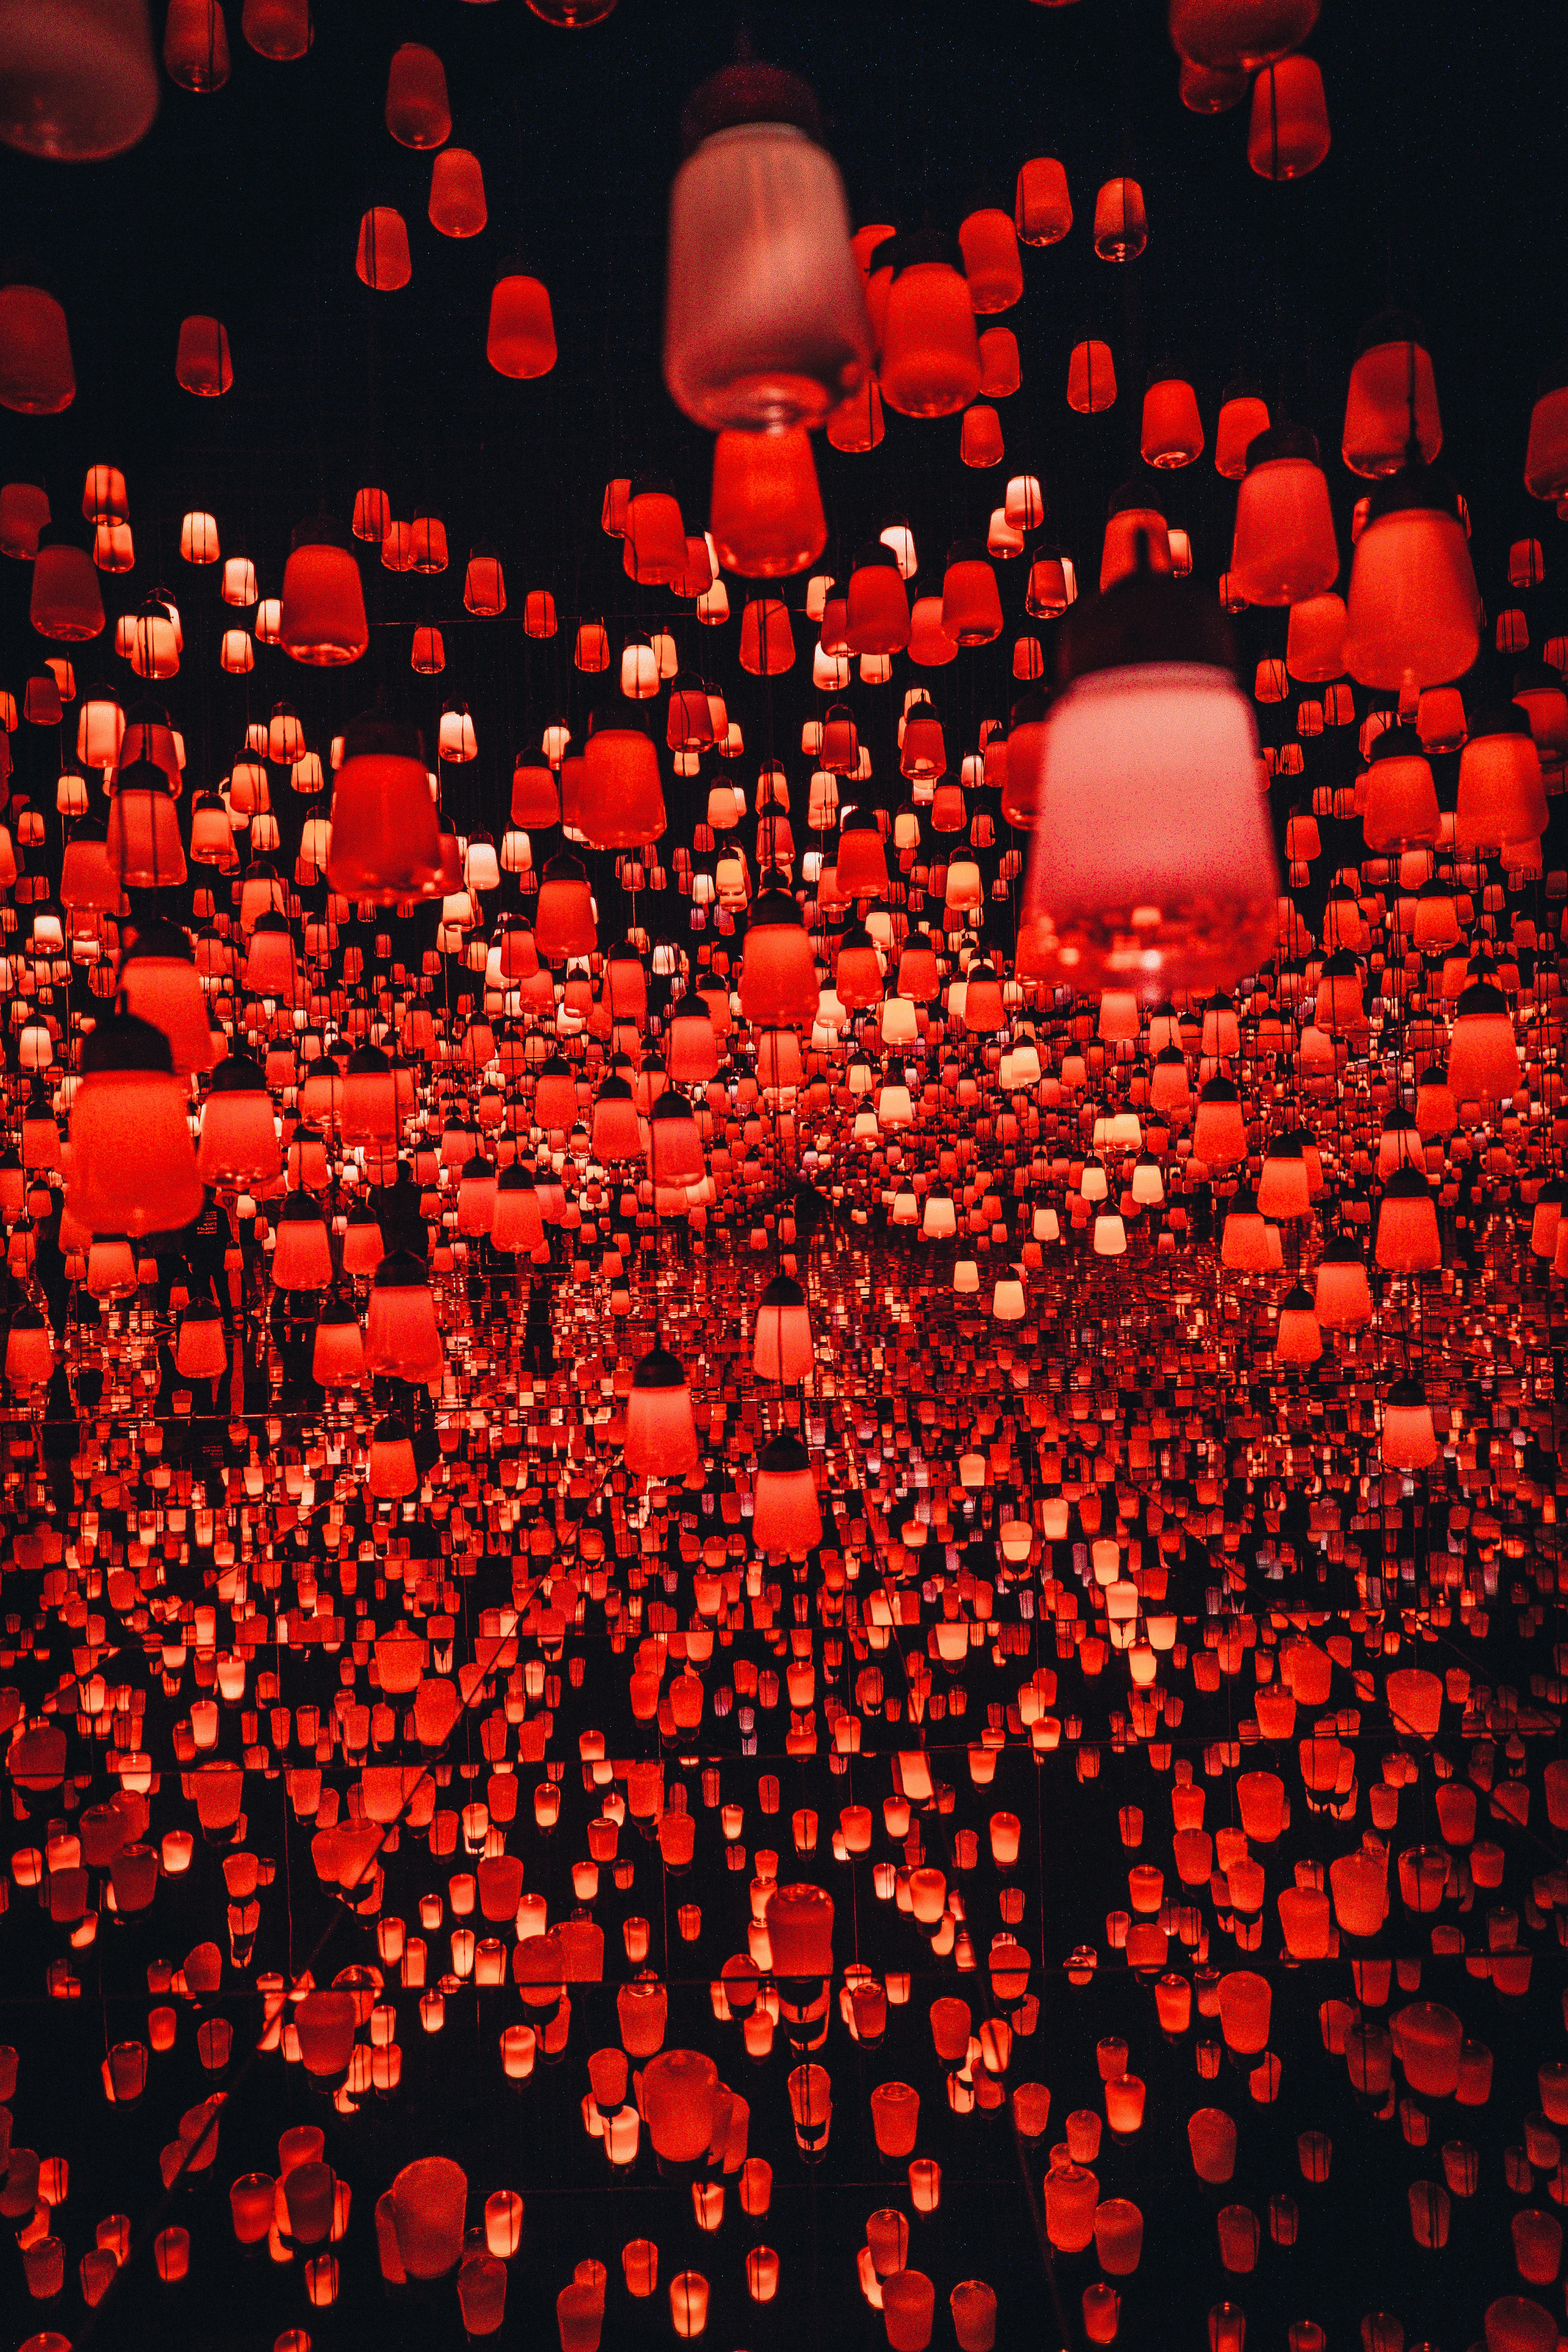
\includegraphics[width=6cm]{Figures/logo}}  %NEW: Changing logo
\def\extraspace{\vspace*{1.6cm}}
\makeatletter
\def\contactdetails{\faicon{phone} & \@telephone \\
                    \faicon{envelope} & \@email}
\makeatother

%%%% FRONT PAGE OF REPORTS

\def\reporttype{Report for}

\long\def\front#1#2#3{
\newpage
\begin{singlespacing}
\thispagestyle{empty}
\vspace*{-1.4cm}
\hspace*{-1.4cm}
\hbox to 16cm{
  \hbox to 6.5cm{\vbox to 14cm{\vbox to 25cm{
    \logo
    \vfill
    \parbox{6.3cm}{\raggedright
      \sf\color[rgb]{0.8, 0.7, 0.1 }    % NEW color 
      {\large\textbf{\name}}\par
      \vspace{.7cm}
      \tabcolsep=0.12cm\sf\small
      \begin{tabular}{@{}ll@{}}\contactdetails
      \end{tabular}
      \vspace*{0.3cm}\par
      ABN: \abn\par
    }
  }\vss}\hss}
  \hspace*{0.2cm}
  \hbox to 1cm{\vbox to 14cm{\rule{4pt}{26.8cm}\vss}\hss\hfill}  %NEW: Thicker line
  \hbox to 10cm{\vbox to 14cm{\vbox to 25cm{   
      \vspace*{3cm}\sf\raggedright
      \parbox{11cm}{\sf\raggedright\baselineskip=1.2cm
         \fontsize{24.88}{30}\color[rgb]{0, 0.29, 0.55}\sf\textbf{#1}}   % NEW: title color blue
      \par
      \vfill
      \large
      \vbox{\parskip=0.8cm #2}\par
      \vspace*{2cm}\par
      \reporttype\\[0.3cm]
      \hbox{#3}%\\[2cm]\
      \vspace*{1cm}
      {\large\sf\textbf{\Date~\Month~\Year}}
   }\vss}
  }}
\end{singlespacing}
\newpage
}

\makeatletter
\def\titlepage{\front{\expandafter{\@title}}{\@author}{\@organization}}
\makeatother

\usepackage{setspace}
\setstretch{1.5}

%% Any special functions or other packages can be loaded here.
\usepackage{booktabs}
\usepackage{longtable}
\usepackage{array}
\usepackage{multirow}
\usepackage{wrapfig}
\usepackage{float}
\usepackage{colortbl}
\usepackage{pdflscape}
\usepackage{tabu}
\usepackage{threeparttable}
\usepackage{threeparttablex}
\usepackage[normalem]{ulem}
\usepackage{makecell}
\usepackage{xcolor}


\begin{document}
\titlepage

\hypertarget{introduction}{%
\section{Introduction}\label{introduction}}

\hypertarget{library-used}{%
\section{Library used}\label{library-used}}

The library packages used in our research consist of:

\begin{itemize}
\tightlist
\item
  tidyverse (\textcite{tidyverse})
\item
  readr (\textcite{readr})
\item
  kableExtra (\textcite{kableExtra})
\item
  Bookdown (\textcite{bookdown} \textcite{bookdown1})
\item
  gridExtra (\textcite{gridExtra})
\item
  Tinytex (\textcite{tinytex} \textcite{tinytex1})
\item
  Knitr (\textcite{knitr} \textcite{knitr1})
\end{itemize}

\clearpage

\section*{}

\hypertarget{yanchuilucia_cheung}{%
\subsection{YanChuiLucia\_Cheung}\label{yanchuilucia_cheung}}

\hypertarget{research-question}{%
\subsubsection{research question}\label{research-question}}

-1. How is the trend of \textbf{malaria} change across the years in the WORLD ?

-2. What is the 5 countries with highest death rates for malaria

-3. What is the preventive measures for malaria?

Malaria is a parasitic disease caused by Anopheles mosquitoes, the main types of parasite that are found in infected population are Plasmodium
falciparum or Plasmodium vivax (\textcite{malariaintro}).

\begin{figure}
\includegraphics[width=0.7\linewidth]{report_files/figure-latex/worldtrend-1} \caption{Malaria world trend}\label{fig:worldtrend}
\end{figure}

Figure \ref{fig:worldtrend} shows the world trend of malaria death rate across 2000 to 2019. The downward trend could be the result of two reasons. Firstly, the increase in malaria program funding from 960 million US dollar in 2005 to 2.5 billion US dollar in 2014 (\textcite{MalariaTrend}). Secondly, World Health Organisation (WHO) updated the strategies for malaria in 2010s, ensure it is efficient from time to time to control malaria transmission and increase in financial support for malaria researches in the early 2000s (\textcite{MalariaTrend2}).

\begin{table}

\caption{\label{tab:countries}Top 5 Countries with highest Malaria death rate}
\centering
\begin{tabular}[t]{l|r}
\hline
Country & Mean\\
\hline
Nigeria & 230503\\
\hline
Democratic Republic of Congo & 84195\\
\hline
India & 56857\\
\hline
Uganda & 38987\\
\hline
Burkina Faso & 35718\\
\hline
\end{tabular}
\end{table}

Table \ref{tab:countries} lists the top 5 countries with highest Malaria death rate. By comparing the mean death rate, the data of Nigeria is significantly higher than other countries.

\begin{figure}[H]
\includegraphics[width=0.7\linewidth]{report_files/figure-latex/countrygraph-1} \caption{Top 5 countries with the highest malaria death rate}\label{fig:countrygraph}
\end{figure}

Figure \ref{fig:countrygraph} shows the death rate trend by countries from 2000 to 2019. Overall, the trend was decreasing over the years with fluctuations in some of the countries. The reason for the downward trend could be the increase in the population with the access of insecticide-treated net in malaria prevalent countries from 7\% to 67\% in 2015 (\textcite{MalariaTrend}).

There are mainly 2 reasons causing the high death rate in these countries. These countries have hot and humid weather. Temperature higher or equal to 21℃ is the most suitable condition for one of the fatal malaria parasites to grow into vector (\textcite{climate}). The average temperature in Nigeria can be up to 40 degree Celsius and annual rainfall can up to 4000mm, these conditions create suitable environment for malaria parasite (\textcite{Nigeria} and \textcite{climate}).

Secondly, these countries lack comprehensive report system. Only a small proportion of malaria cases is reported to government in Nigeria (\textcite{Nigeria2}). People living in that area who are not infected may not be able to take precaution or aware of the disease as the actual number of confirmed cases could be higher than the reported cases. In India, hospitals and clinics do not report malaria cases to corresponding government organisation (\textcite{India}).

More than 100 countries have eliminated malaria, and one third of the remaining countries has been actively fighting malaria (\textcite{precautions}). Some of the preventive measures taken by these countries could be the reference for the 5 countries mentioned above. In Maldives, every confirmed malaria case must report to government (\textcite{India}). In Sri Lanka, mobile malaria clinic was set up to identify people who infected malaria in early stage, patients can receive proper treatment before the symptoms become severe (\textcite{India}).

There are some precautions that are widely used in malaria prevalent countries, such as insecticide and insecticide-treated net to prevent mosquito bite (\textcite{malariaintro}). Lastly, the RTS,S subunit vaccine could be a hope for population who are suffering from malaria. Even though the vaccine is still in testing stage, it has approved by World Health Organisation (\textcite{Vaccine}).

\section*{}

\hypertarget{minmin_soh}{%
\subsection{MinMin\_Soh}\label{minmin_soh}}

\hypertarget{deaths---hivaids}{%
\subsection{Deaths - HIV/AIDS}\label{deaths---hivaids}}

Research Questions:

\begin{itemize}
\tightlist
\item
  How is the death rates of \textbf{HIV / AIDS} change in the world ?
\item
  What is the top 5 countries with the highest death rates from \textbf{HIV / AIDS} and the death trends for those countries?
\item
  What are the preventive measures for \textbf{HIV / AIDS} ?
\end{itemize}

\clearpage

\hypertarget{hivaids}{%
\subsubsection{HIV/AIDS}\label{hivaids}}

\textcite{cai2009stability} discussed tt is estimated that 38.6 million population is currently living with HIV infection. After several infection stages, AIDS would be developed.

\hypertarget{death-rates-of-hiv-aids-in-the-world}{%
\subsubsection{\texorpdfstring{Death rates of \textbf{HIV / AIDS} in the world}{Death rates of HIV / AIDS in the world}}\label{death-rates-of-hiv-aids-in-the-world}}

\begin{figure}
\centering
\includegraphics{report_files/figure-latex/WorldHIVtrend-1.pdf}
\caption{\label{fig:WorldHIVtrend}Number of Deaths from HIV/AIDS in the World}
\end{figure}

Figure \ref{fig:WorldHIVtrend} depicts the global death rate of HIV/AIDS over time. As observed, the death rate followed an increasing trend from 1990 to around 2005, and then decreased from 2005 onwards.

\clearpage

\hypertarget{the-5-countries-with-the-highest-death-rates-from-hiv-aids}{%
\subsubsection{\texorpdfstring{The 5 countries with the highest death rates from \textbf{HIV / AIDS}}{The 5 countries with the highest death rates from HIV / AIDS}}\label{the-5-countries-with-the-highest-death-rates-from-hiv-aids}}

\begin{table}[!h]

\caption{\label{tab:HIVtable}Top 5 countries with the highest average death rates from HIV / AIDS}
\centering
\begin{tabular}[t]{lr}
\toprule
Entity & Average Death Rates from HIV/AIDS\\
\midrule
\cellcolor{gray!6}{South Africa} & \cellcolor{gray!6}{162477}\\
Kenya & 86118\\
\cellcolor{gray!6}{Tanzania} & \cellcolor{gray!6}{82168}\\
India & 81812\\
\cellcolor{gray!6}{Nigeria} & \cellcolor{gray!6}{73891}\\
\bottomrule
\end{tabular}
\end{table}

Table \ref{tab:HIVtable} above depicts the 5 countries with the highest average death rates from HIV / AIDS from year 1990 to year 2019. South Africa had the highest average death rate, followed by Kenya, Tanzania, India and Nigeria.

\hypertarget{the-death-trends-for-the-5-countries-with-the-highest-average-death-rates-from-hivaids}{%
\subsubsection{The death trends for the 5 countries with the highest average death rates from HIV/AIDS}\label{the-death-trends-for-the-5-countries-with-the-highest-average-death-rates-from-hivaids}}

Figure \ref{fig:HIVtrend} depicts the death rates from HIV/AIDS for the 5 countries listed in the table above. Each country appears to follow the global death rate trend of increasing from the 1990s to the 2000s, before decreasing from 2005 to 2020. This is highly evident in South Africa and India.

\begin{figure}
\centering
\includegraphics{report_files/figure-latex/HIVtrend-1.pdf}
\caption{\label{fig:HIVtrend}Top 5 countries with the highest average death rates from HIV/AIDS}
\end{figure}

\clearpage

\hypertarget{preventive-measures-for-hiv-aids}{%
\subsubsection{\texorpdfstring{Preventive measures for \textbf{HIV / AIDS}}{Preventive measures for HIV / AIDS}}\label{preventive-measures-for-hiv-aids}}

\begin{itemize}
\tightlist
\item
  \emph{Antiretroviral Therapy (ART)}
\end{itemize}

ART treatment involves taking medicines to slow down HIV multiplication rate to prevent HIV from progressing to AIDS, and therefore provide longer lives for patients as discussed in \textcite{kemnic2018hiv}. Figure \ref{fig:ARTplot} depicts the rate of HIV/AIDS-related deaths averted due to ART. \textcite{sashindran2016antiretroviral} and \textcite{world2006towards} explained that although the treatment was developed in the 1980s, it wasn't widely available in developing countries such as India until the WHO enacted the 3 by 5 initiative between 2003 and 2005. Therefore, figure \ref{fig:ARTplot} shows an rising trend of HIV/AIDS-related deaths since 2005, which means that the treatment is effective in slowing HIV/AIDS-related deaths.

This increased the use of ART around the world to treat HIV/AIDS since 2005 can also explain why each country above follows an increasing trend from the mid 2000s.

\begin{figure}
\centering
\includegraphics{report_files/figure-latex/ARTplot-1.pdf}
\caption{\label{fig:ARTplot}Effectiveness of Antiretroviral therapy on HIV / AIDS over the years}
\end{figure}

\clearpage

\begin{itemize}
\tightlist
\item
  \emph{Contraception measures}
\end{itemize}

To further prevent HIV/AIDS, contraception needs to be `at the centre of the HIV prevention agenda', as discussed in \textcite{crankshaw2016placing}. \textcite{newell1998mechanisms} explained that this not only protects people from getting HIV/AIDS but also newborn babies, as HIV/AIDS can be transmitted from mothers to their newborn children.

\begin{itemize}
\tightlist
\item
  \emph{Education}
\end{itemize}

Education also needs to be at the forefront of preventive measures as many people in developing countries are unaware of preventative measures for HIV/AIDS, \textcite{baxen2004researching}.

\section*{}

\hypertarget{sanna_meer}{%
\subsection{Sanna\_Meer}\label{sanna_meer}}

\section*{}

\hypertarget{aphiaut_imuan}{%
\subsection{Aphiaut\_Imuan}\label{aphiaut_imuan}}

\clearpage

\hypertarget{conclusion}{%
\section{Conclusion :}\label{conclusion}}

\clearpage

\clearpage

\section*{}

\hypertarget{sanna_meer-1}{%
\subsection{Sanna\_Meer}\label{sanna_meer-1}}

\section*{Deaths - Cardiovascular diseases}

\hypertarget{aphiaut_imuan-1}{%
\subsection{Aphiaut\_Imuan}\label{aphiaut_imuan-1}}

The research question for analysis in this section are :\\
- How is \textbf{the trend of Cardiovascular diseases} changed across the years in the \textbf{world}?
- What are \textbf{the 5 countries with the highest death} from Cardiovascular diseases?
- What are the healthy lifestyle factors for Cardiovascular diseases?

\begin{figure}[H]

{\centering \includegraphics[width=0.8\linewidth]{report_files/figure-latex/worldtrendcardio-1} 

}

\caption{The trend of Cardiovascular diseases in the world}\label{fig:worldtrendcardio}
\end{figure}

\begin{table}[!h]

\caption{\label{tab:tabletop5cardio}The top 5 countries by death of Cardiovascular diseases}
\centering
\begin{tabular}[t]{l|r|r}
\hline
country & mean & max\\
\hline
China & 3350199.1 & 4584273\\
\hline
India & 1766490.3 & 2574410\\
\hline
Russia & 1130126.0 & 1338945\\
\hline
United States & 881278.2 & 957455\\
\hline
Indonesia & 452900.4 & 651481\\
\hline
\end{tabular}
\end{table}

\begin{figure}[H]

{\centering \includegraphics[width=0.8\linewidth]{report_files/figure-latex/graphtop5cardio-1} 

}

\caption{The 5 countries with the highest death from Cardiovascular diseases}\label{fig:graphtop5cardio}
\end{figure}

The number of deaths from cardiovascular diseases from 1990 to 2019 in Figure \ref{fig:worldtrendcardio} shows a significantly positive trend and is likely to continue to increase. Table \ref{tab:tabletop5cardio} illustrates the top 5 countries with the highest death from cardiovascular diseases including China, India, Russia, the United States, and Indonesia, respectively. Moreover, \textcite{zhang_2021_healthy} investigated people dying from cardiovascular disease in China are described by the high-salt food, high cholesterol, and high smoking rate. \textcite{yang_2015_cardiovascular} argue that around 17\% of the number of death by cardiovascular diseases were due to ambient temperature and the number of death from cold temperatures more than heat temperatures. These studies can support the result of China in Figure \ref{fig:graphtop5cardio}.
Furthermore, figure 2 shows India and Indonesia are positive trend like China because 35 \% of Indian adults are smoking (\textcite{prabhakaran_2016_cardiovascular}) and 26.6 \% of Indonesian adults aged 40 years (\textcite{maharani_2019_cardiovascular}).

In the contrast, Russia has decreasing trend since 2005 because Russia has National Priority Project `Health' to increase the modern treatment and prevention of cardiovascular diseases (\textcite{pogosova_2016_positive}). Moreover, the proportions of smokers in Russia are less than 50 percent which makes the decreasing trend in the number of deaths in Russia (\textcite{lakunchykova_2020_why}). Furthermore, \textcite{zhang_2021_healthy} investigate healthy lifestyle factors such as non-smoking, exercise, eating some healthy food, and don't drink alcohol can reduce the mortality rate of cardiovascular in the USA that is related with our result that the trend of death starts to decrease around 2004. However, it will back to increase because some US populations have been unable access to cardiovascular treatment(\textcite{mensah_2017_decline}).

Above mention, the trend of cardiovascular diseases is increasing trend or decreasing trend depends on the organization of preventing cardiovascular in each country and healthy lifestyle factors of people, such as smoking, exercise, healthy eating, and drinking alcohol.

\clearpage

\hypertarget{conclusion-1}{%
\section{Conclusion :}\label{conclusion-1}}

Cardiovascular part

The government should create a project or have some organization to support and prevent cardiovascular diseases. Moreover, they should make a policy for people to reduce or stop smoking such as increasing the tax on cigarettes for making people can't afford cigarettes.

Malarir part:
Countries with high malaria death rate should establish a reporting system, so that every case is traceable, hence population living in malaria prevalent area can take precautions immediately.

The world is making progress on HIV/AIDS death prevention, demonstrated by the decreasing death rates. Antiretroviral treatment (HRT) has been the key to avert deaths from HIV/AIDS. Strict adherence to other measures including contraception and education can dramatically slow the disease's progress and prevent secondary infections.

\clearpage

© 2022 GitHub, Inc.
Terms
Privacy
Security
Status
Docs
Contact GitHub
Pricing
API
Training
Blog
About

\printbibliography

\end{document}
